\subsection{旋度算子及相关空间}
\label{sec:chap4-curl-spaces}

\renewcommand{\thestatement}{4.\arabic{statement}}
\renewcommand{\theHstatement}{ch04.sec04.\arabic{statement}}
\setcounter{statement}{0}
\renewcommand{\thefigure}{IV.\arabic{figure}}
\renewcommand{\theHfigure}{ch04.\arabic{figure}}
\setcounter{figure}{0}
\newcounter{chapterfoursectionfourremark}
\renewcommand{\thechapterfoursectionfourremark}{4.\arabic{chapterfoursectionfourremark}}

本节的全部材料都在空间维数为 $3$ 的情形下给出, 因为这是定义旋度算子的自然框架. 不过, 通过调整该算子的定义, 大多数结果都可以转移到二维情形; 事实上, 在二维情形中需要定义两个不同的类旋度算子, 一个从 $\mathbb R^2$ 到 $\mathbb R$, 另一个从 $\mathbb R$ 到 $\mathbb R^2$.

我们选择只关注本书后文所需的主要结果. 更多结果可以在文献\MBUnresolvedReference{bib:curl-spaces-references}{[54, 65, 47, 6, 60]}中找到. 我们关心的主要性质由 Theorem~\ref{thm:chap4-vector-potential} 给出: 它断言, 在适当假设下, $(H^1(\Omega))^3$ 中的无散度向量场可以写成 $(H^2(\Omega))^3$ 中某个向量势场的旋度. 这个结果对于研究 Chapter~\MBUnresolvedReference{chap:steady-navier-stokes}{V} 的 Section~\MBUnresolvedReference{sec:steady-navier-stokes-nonhomogeneous}{3} 中带非齐次边界条件的稳态 Navier--Stokes 方程特别有用.

记
\[
 S^2=\{x\in\mathbb R^3,\ |x|=1\}
\]
为 $\mathbb R^3$ 的单位球面. 回忆这个球面是单连通的 (而 $\mathbb R^2$ 的单位球面不是). 这意味着 $S^2$ 上任意连续闭曲线都可以连续变形成一个点.

\subsubsection{Poincaré 定理}
\label{subsec:chap4-poincare-theorems}

本小节证明一些结果, 它们是著名 Poincaré 定理的简单版本; 该定理断言, 星形区域中的任意闭微分形式都是恰当微分形式.

\begin{Lemma}
\label{lem:chap4-poincare-star-shaped}
设 $U\subset\mathbb R^3$ 是关于原点星形的开集, $k\geq1$ 是整数.
\begin{enumerate}
 \item 对任意满足 $\operatorname{curl}\Phi=0$ 于 $U$ 的 $\Phi\in(C^k(U))^3$, 公式
 \begin{equation}
  \psi(x)=\int_0^1\Phi(tx)\cdot x\,\mathrm dt
  \label{eq:chap4-poincare-scalar-potential}
 \end{equation}
 定义函数 $\psi\in C^{k+1}(U)$, 使得 $\Phi=\nabla\psi$.
 \item 对任意满足 $\operatorname{div}\Phi=0$ 于 $U$ 的 $\Phi\in(C^k(U))^3$, 公式
 \[
  \Psi(x)=\int_0^1t\Phi(tx)\wedge x\,\mathrm dt
 \]
 定义函数 $\Psi\in(C^k(U))^3$, 使得 $\Phi=\operatorname{curl}\Psi$.
\end{enumerate}
\end{Lemma}

若 $U$ 关于非原点的某个点星形, 则通过平移即可容易地修改上述公式.

\begin{Proof}
\begin{enumerate}
 \item 式\eqref{eq:chap4-poincare-scalar-potential}显然定义了 $C^k(U)$ 中的函数. 计算其梯度:
 \[
  \begin{aligned}
  \frac{\partial\psi}{\partial x_i}
  &=\int_0^1\frac{\partial\Phi}{\partial x_i}(tx)\cdot xt\,\mathrm dt
    +\int_0^1\Phi(tx)\cdot e_i\,\mathrm dt\\
  &=\sum_{j=1}^3\int_0^1\frac{\partial\Phi_j}{\partial x_i}(tx)x_jt\,\mathrm dt
    +\int_0^1\Phi_i(tx)\,\mathrm dt.
  \end{aligned}
 \]
 由于 $\operatorname{curl}\Phi=0$, 有 $\partial\Phi_j/\partial x_i=\partial\Phi_i/\partial x_j$, 因而
 \[
  \begin{aligned}
  \frac{\partial\psi}{\partial x_i}
  &=\sum_{j=1}^3\int_0^1\frac{\partial\Phi_i}{\partial x_j}(tx)x_jt\,\mathrm dt
    +\int_0^1\Phi_i(tx)\,\mathrm dt\\
  &=\int_0^1\frac{\mathrm d}{\mathrm dt}\bigl(t\Phi_i(tx)\bigr)\,\mathrm dt
   =\Phi_i(x).
  \end{aligned}
 \]
 所以 $\nabla\psi=\Phi$, 且 $\psi\in C^{k+1}(U)$.

 \item 设 $i,j,k\in\{1,2,3\}$ 满足 $e_i\wedge e_j=e_k$. 需要证明
 \[
  \Phi_k=\frac{\partial\Psi_j}{\partial x_i}
  -\frac{\partial\Psi_i}{\partial x_j}.
 \]
 为此写成
 \[
  \Psi_i(x)=\int_0^1\bigl(tx_k\Phi_j(tx)-tx_j\Phi_k(tx)\bigr)\,\mathrm dt,
 \]
 于是
 \[
  \frac{\partial\Psi_i}{\partial x_j}(x)
  =\int_0^1\left(
  t^2x_k\frac{\partial\Phi_j}{\partial x_j}(tx)
  -t^2x_j\frac{\partial\Phi_k}{\partial x_j}(tx)
  -t\Phi_k(tx)\right)\,\mathrm dt.
 \]
 类似地,
 \[
  \frac{\partial\Psi_j}{\partial x_i}(x)
  =\int_0^1\left(
  -t^2x_k\frac{\partial\Phi_i}{\partial x_i}(tx)
  +t^2x_i\frac{\partial\Phi_k}{\partial x_i}(tx)
  +t\Phi_k(tx)\right)\,\mathrm dt.
 \]
 因而
 \[
  \begin{aligned}
  \frac{\partial\Psi_j}{\partial x_i}(x)
  -\frac{\partial\Psi_i}{\partial x_j}(x)
  ={}&\int_0^1-t^2x_k\left(
  \frac{\partial\Phi_i}{\partial x_i}(tx)
  +\frac{\partial\Phi_j}{\partial x_j}(tx)\right)\,\mathrm dt\\
  &+\int_0^1\left(
  t^2x_j\frac{\partial\Phi_k}{\partial x_j}(tx)
  +t^2x_i\frac{\partial\Phi_k}{\partial x_i}(tx)
  +2t\Phi_k(tx)\right)\,\mathrm dt.
  \end{aligned}
 \]
 由于 $\operatorname{div}\Phi=0$, 有
 \[
  \frac{\partial\Phi_i}{\partial x_i}
  +\frac{\partial\Phi_j}{\partial x_j}
  =-\frac{\partial\Phi_k}{\partial x_k},
 \]
 从而
 \[
  \begin{aligned}
  \frac{\partial\Psi_j}{\partial x_i}(x)
  -\frac{\partial\Psi_i}{\partial x_j}(x)
  &=\int_0^1\bigl(t^2x\cdot\nabla\Phi_k(tx)+2t\Phi_k(tx)\bigr)\,\mathrm dt\\
  &=\int_0^1\frac{\mathrm d}{\mathrm dt}\bigl(t^2\Phi_k(tx)\bigr)\,\mathrm dt
  =\Phi_k(x).
  \end{aligned}
 \]
 最终已经证明 $\operatorname{curl}\Psi=\Phi$.
\end{enumerate}
\end{Proof}

\begin{Lemma}
\label{lem:chap4-poincare-simply-connected}
设 $\Omega$ 是 $\mathbb R^3$ 中单连通的开集, $k\geq1$ 是整数. 对任意满足 $\operatorname{curl}\Phi=0$ 于 $\Omega$ 的 $\Phi\in(C^k(\Omega))^3$, 存在 $\psi\in(C^{k+1}(\Omega))^3$, 使得 $\Phi=\nabla\psi$.
\end{Lemma}

\begin{Proof}
设 $x_0\in\Omega$. 定义 $U$ 为包含 $x_0$ 且包含于 $\Omega$ 的最大连通开集, 在 $U$ 上存在这样的函数 $\psi$. 由 Lemma~\ref{lem:chap4-poincare-star-shaped}, 已知 $U$ 非空, 因为在包含于 $\Omega$ 且以 $x_0$ 为中心的任意球中都能找到这样的 $\psi$. 记 $\psi\in C^{k+1}(U)$ 满足 $\Phi=\nabla\psi$ 于 $U$.

现在用反证法证明 $U=\Omega$.
\begin{itemize}
 \item 假设 $V=\Omega\setminus U$ 非空; 则 $\partial U\cap V\neq\varnothing$. 事实上, 若 $\partial U\cap V$ 为空, 就有 $V=\Omega\setminus\overline U$, 因而 $V$ 是开集. 于是 $\Omega=U\cup V$ 且 $U\cap V=\varnothing$, 但这与 $\Omega$ 连通矛盾.

 取 $x\in\partial U\cap V$, 并取以 $x$ 为中心且包含于 $\Omega$ 的球 $B$. 由于 $x\in\partial U$, 有 $U\cap B\neq\varnothing$, 因而可取一点 $\widetilde x\in U\cap B$.

 \item 由 Lemma~\ref{lem:chap4-poincare-star-shaped}, 存在 $\widetilde\psi\in C^{k+1}(B)$ 使得 $\Phi=\nabla\widetilde\psi$ 于 $B$; 可以给 $\widetilde\psi$ 加上一个常数, 使 $\widetilde\psi(\widetilde x)=\psi(\widetilde x)$.

 \item 现在证明 $\psi=\widetilde\psi$ 于 $U\cap B$. 设 $y$ 是 $U\cap B$ 中任意一点. 由于 $U$ 是连通开集, 存在 $C^2$ 路径 $\gamma_0:[0,1]\to U$, 满足 $\gamma_0(0)=\widetilde x$ 且 $\gamma_0(1)=y$. 类似地, 存在 $C^2$ 路径 $\gamma_1:[0,1]\to B$, 满足 $\gamma_1(0)=\widetilde x$ 且 $\gamma_1(1)=y$.

 由于区域 $\Omega$ 是开且单连通的, 存在 $C^2$ 映射 $\gamma:[0,1]\times[0,1]\to\Omega$, 满足
 \[
  \gamma(0,\cdot)=\gamma_0,\quad
  \gamma(1,\cdot)=\gamma_1,\quad
  \gamma(\cdot,0)=\widetilde x,\quad
  \gamma(\cdot,1)=y.
 \]
 定义
 \[
  I(s)=\int_0^1\Phi(\gamma(s,t))\cdot\partial_t\gamma(s,t)\,\mathrm dt,
  \qquad\forall s\in[0,1].
 \]
 对 $s=0$, $\gamma(0,\cdot)=\gamma_0$ 是 $U$ 中的路径, 因而
 \[
  \begin{aligned}
  I(0)
  &=\int_0^1\Phi(\gamma_0(t))\cdot\gamma_0'(t)\,\mathrm dt
   =\int_0^1(\nabla\psi)(\gamma_0(t))\cdot\gamma_0'(t)\,\mathrm dt\\
  &=\psi(\gamma_0(1))-\psi(\gamma_0(0))
   =\psi(y)-\psi(\widetilde x).
  \end{aligned}
 \]
 对 $s=1$, $\gamma(1,\cdot)=\gamma_1$ 是 $B$ 中的路径, 因而
 \[
  \begin{aligned}
  I(1)
  &=\int_0^1\Phi(\gamma_1(t))\cdot\gamma_1'(t)\,\mathrm dt
   =\int_0^1(\nabla\widetilde\psi)(\gamma_1(t))\cdot\gamma_1'(t)\,\mathrm dt\\
  &=\widetilde\psi(\gamma_1(1))-\widetilde\psi(\gamma_1(0))
   =\widetilde\psi(y)-\widetilde\psi(\widetilde x).
  \end{aligned}
 \]
 计算导数 $I'(s)$:
 \[
  \begin{aligned}
  I'(s)
  ={}&\int_0^1\bigl((\nabla\Phi)(\gamma(s,t))\cdot\partial_s\gamma(s,t)\bigr)
  \cdot\partial_t\gamma(s,t)\,\mathrm dt\\
  &+\int_0^1\Phi(\gamma(s,t))\cdot\partial_s\partial_t\gamma(s,t)\,\mathrm dt.
  \end{aligned}
 \]
 条件 $\operatorname{curl}\Phi=0$ 蕴含矩阵 $\nabla\Phi$ 对称, 因而
 \[
  \begin{aligned}
  I'(s)
  ={}&\int_0^1\bigl((\nabla\Phi)(\gamma(s,t))\cdot\partial_t\gamma(s,t)\bigr)
  \cdot\partial_s\gamma(s,t)\,\mathrm dt\\
  &+\int_0^1\Phi(\gamma(s,t))\cdot\partial_s\partial_t\gamma(s,t)\,\mathrm dt\\
  &=\int_0^1\frac{\mathrm d}{\mathrm dt}
  \bigl(\Phi(\gamma(s,t))\cdot\partial_s\gamma(s,t)\bigr)\,\mathrm dt\\
  &=\Phi(\gamma(s,1))\cdot\partial_s\gamma(s,1)
  -\Phi(\gamma(s,0))\cdot\partial_s\gamma(s,0)=0,
  \end{aligned}
 \]
 因为映射 $s\mapsto\gamma(s,1)$ 和 $s\mapsto\gamma(s,0)$ 都是常值映射.

 所以上述计算给出 $I(0)=I(1)$; 即
 \[
  \widetilde\psi(y)-\widetilde\psi(\widetilde x)
  =\psi(y)-\psi(\widetilde x).
 \]
 按构造 $\psi(\widetilde x)=\widetilde\psi(\widetilde x)$, 因而推出 $\psi(y)=\widetilde\psi(y)$.

 \item 已经证明 $\psi=\widetilde\psi$ 于 $U\cap B$, 因而在 $U\cup B$ 上定义的映射
 \[
  \psi=\begin{cases}
  \psi,&\text{on }U,\\
  \widetilde\psi,&\text{on }B
  \end{cases}
 \]
是良定义且光滑的, 并满足 $\nabla\psi=\Phi$ 于开连通集 $U\cup B$. 这与 $U$ 的极大性假设矛盾.
\end{itemize}
\end{Proof}

\begin{Lemma}
\label{lem:chap4-poincare-compact-vector-potential}
设 $U\subset\mathbb R^3$ 是关于原点星形的开集, $k\geq1$ 是整数. 对任意满足 $\operatorname{div}\Phi=0$ 的 $\Phi\in(C_c^k(U))^3$, 存在 $\Psi\in(C_c^k(U))^3$, 使得 $\Phi=\operatorname{curl}\Psi$.
\end{Lemma}

\begin{Proof}
由于 $\Phi$ 紧支撑, 不失一般性可以假设 $U$ 有界; 此时由 Lemma~\ref{lem:chap4-poincare-star-shaped}, 已知存在 $\widetilde\Psi\in(C^k(U))^3$, 使得 $\Phi=\operatorname{curl}\widetilde\Psi$ 于 $U$, 但 $\widetilde\Psi$ 不一定紧支撑.

取关于 $0$ 星形且包含 $\Phi$ 的支撑的开集 $U_0$, 使 $U_0\subset\overline U_0\subset U$. 按构造, $\operatorname{curl}\widetilde\Psi=0$ 于 $U\setminus\overline U_0$.

注意存在两个连续映射 $\xi_0,\xi:S^2\to]0,+\infty[$, 满足 $\xi_0<\xi$, 并且
\[
 U_0=\left\{x\in\mathbb R^3,\ |x|<\xi_0\left(\frac{x}{|x|}\right)\right\},
 \qquad
 U=\left\{x\in\mathbb R^3,\ |x|<\xi\left(\frac{x}{|x|}\right)\right\}.
\]
特别地, 集合 $U_0'=U\setminus\overline U_0$ 满足
\[
 U_0'=\left\{x\in\mathbb R^3,
 \ \xi_0\left(\frac{x}{|x|}\right)<|x|<
 \xi\left(\frac{x}{|x|}\right)\right\},
\]
因而同胚于 $S^2\times]0,1[$. 所以 $U_0'$ 单连通. 由 Lemma~\ref{lem:chap4-poincare-simply-connected}, 存在 $\widetilde\psi\in C^{k+1}(U_0')$, 使得 $\widetilde\Psi=\nabla\widetilde\psi$ 于 $U_0'$.

任取关于 $0$ 星形的开集 $U_1$, 使 $U_0\subset\overline U_0\subset U_1\subset\overline U_1\subset U$. 可以找到 $\psi\in C^{k+1}(U)$, 使得 $\psi=\widetilde\psi$ 于 $U\setminus U_1$; 现在定义 $\Psi=\widetilde\Psi-\nabla\psi$.

按构造, $\operatorname{curl}\Psi=\Phi$ 于 $U$, 且 $\Psi=0$ 于 $U\setminus U_1$, 结论得证.
\end{Proof}
\subsubsection{空间 $H_{\operatorname{curl}}(\Omega)$}
\label{subsec:chap4-hcurl-space}

现在可以研究旋度算子起关键作用的一些函数空间, 正如在 Subsection~\ref{subsec:chap4-hdiv-space} 中对空间 $H_{\operatorname{div}}(\Omega)$ 所做的那样.

\paragraph{定义和初步性质}

\begin{Definition}
\label{def:chap4-hcurl-space}
设 $\Omega$ 是 $\mathbb R^3$ 中边界紧的 Lipschitz 区域. 定义空间
\[
 H_{\operatorname{curl}}(\Omega)
 =\{u\in(L^2(\Omega))^3,\ \operatorname{curl}u\in(L^2(\Omega))^3\},
\]
并赋予范数
\[
 \|u\|_{H_{\operatorname{curl}}}
 =\bigl(\|u\|_{L^2}^2+\|\operatorname{curl}u\|_{L^2}^2\bigr)^{1/2}.
\]
容易看出, $H_{\operatorname{curl}}(\Omega)$ 是 Hilbert 空间.

此外, 定义 $H_{\operatorname{curl},0}(\Omega)$ 为 $(\mathcal D(\Omega))^3$ 在 $H_{\operatorname{curl}}(\Omega)$ 中的闭包.
\end{Definition}

使用 Chapter~\ref{chap:sobolev-spaces} 的 Section~\ref{subsec:chap3-first-order-operator-domains} 中引入的记号, 可见 $H_{\operatorname{curl}}(\Omega)$ 恰好是旋度算子在 $L^2$ 中的定义域. 更准确地说,
\[
 H_{\operatorname{curl}}(\Omega)=W_{\operatorname{curl}}^{2,2}(\Omega).
\]
于是可以用这个记号重新表述 Chapter~\ref{chap:sobolev-spaces} 的 Section~\ref{subsec:chap3-first-order-operator-domains} 中得到的各个结果:
\begin{itemize}
 \item 空间 $(C_c^\infty(\overline\Omega))^3$ 在 $H_{\operatorname{curl}}(\Omega)$ 中稠密 (见 Theorem~\ref{thm:chap3-graph-space-density}).
 \item 存在从 $H_{\operatorname{curl}}(\Omega)$ 到 $(H^{-1/2}(\partial\Omega))^3$ 的连续迹算子 $\gamma_{\wedge\nu}$, 使对任意 $u\in(C_c^\infty(\overline\Omega))^d$ 有 $\gamma_{\wedge\nu}(u)=u\wedge\nu$. 此外, 成立如下 Stokes 公式:
 \begin{equation}
  \int_\Omega u\cdot(\operatorname{curl}\psi)\,\mathrm dx
  =\int_\Omega(\operatorname{curl}u)\cdot\psi\,\mathrm dx
  +\langle\gamma_{\wedge\nu}(u),\gamma_0(\psi)\rangle_{H^{-1/2},H^{1/2}},
  \quad\forall\psi\in(H^1(\Omega))^3.
  \label{eq:chap4-hcurl-stokes-formula}
 \end{equation}
 这来自 Theorem~\ref{thm:chap3-generalized-normal-trace}. 还要注意, 迹 $\gamma_{\wedge\nu}(u)$ 在如下弱意义下是切向向量场:
 \[
  \langle\gamma_{\wedge\nu}(u),\gamma_0(\psi)\rangle_{H^{-1/2},H^{1/2}}=0,
 \]
对所有满足 $\gamma_0(\psi)\wedge\nu=0$ 的 $\psi\in(H^1(\Omega))^3$ 成立.
 \item 空间 $H_{\operatorname{curl},0}(\Omega)$ 是迹算子 $\gamma_{\wedge\nu}$ 的核 (见 Theorem~\ref{thm:chap3-graph-space-zero-trace}).
\end{itemize}

注意, 对任意函数 $p\in H^1(\Omega)$, 有 $\operatorname{curl}(\nabla p)=0$, 因而 $\nabla p\in H_{\operatorname{curl}}(\Omega)$. 直观上, 可以把 $\nabla p\wedge\nu$ 看作 $p$ 的梯度的切向部分, 所以条件 $\nabla p\wedge\nu=0$ 应当蕴含 $p$ 在 $\Omega$ 的边界上局部为常数. 然而, 由于迹是在弱意义下理解的, 这一点并不明显. 当区域足够光滑时, 下面的命题给出这个性质的详细证明.

\begin{Proposition}
\label{prop:chap4-zero-tangential-gradient-trace}
设 $\Omega$ 是 $\mathbb R^3$ 中 $C^{1,1}$ 类有界区域. 设 $p\in H^1(\Omega)$ 且 $\gamma_{\wedge\nu}(\nabla p)=0$; 则 $\gamma_0(p)$ 在 $\partial\Omega$ 的每个连通分支上都是常数.
\end{Proposition}

\begin{Proof}
由式\eqref{eq:chap4-hcurl-stokes-formula}, 得到
\begin{equation}
 \int_\Omega\nabla p\cdot\operatorname{curl}\psi\,\mathrm dx=0,
 \qquad\forall\psi\in(H^1(\Omega))^3.
 \label{eq:chap4-gradient-curl-orthogonality}
\end{equation}
从这个公式证明 $\gamma_0(p)$ 在 $\partial\Omega$ 上局部为常数, 命题即得证.

任取一点 $x_0\in\partial\Omega$, 并取 $\partial\Omega$ 中 $x_0$ 的两个连通有界开邻域 $\Sigma,\Sigma^*$, 使 $\overline\Sigma\subset\Sigma^*$ (闭包在拓扑空间 $\partial\Omega$ 的意义下理解). 再取任意函数 $g\in C_c^\infty(\Sigma)$, 满足
\[
 \int_{\partial\Omega}g\,\mathrm d\sigma
 =\int_\Sigma g\,\mathrm d\sigma=0.
\]
把 $g$ 在 $\partial\Omega\setminus\Sigma$ 上作零延拓. 如果能够证明对任意这样的 $g$ 都有
\[
 \int_\Sigma\gamma_0(p)g\,\mathrm d\sigma=0,
\]
则结论得证. 事实上, 由此推出 $\gamma_0(p)$ 在 $\Sigma$ 上为常数, 而 $\Sigma$ 是 $\partial\Omega$ 任意一点的开邻域.

使用 Chapter~\ref{chap:sobolev-spaces} 的 Section~\ref{sec:chap3-boundary-calculus} 中的记号和结果. 特别地, 考虑坐标系
\[
 \psi_{s_0}:(\sigma,s)\in\Gamma_{s_0}\times[0,s_0]
 \longmapsto O_{s_0}^\rho,
\]
它可以延拓到 $\Gamma_{s_0}\times[-s_0,s_0]$. 引入
\[
 \Sigma_{s_0}=\psi(\cdot,s_0)^{-1}(\Sigma),
 \qquad
 \Sigma_{s_0}^*=\psi(\cdot,s_0)^{-1}(\Sigma^*),
\]
以及对任意 $\xi_1,\xi_2$ 定义
\[
 U_{\xi_1,\xi_2}=\psi(\Sigma_{s_0}\times]\xi_1,\xi_2[),
 \qquad
 U_{\xi_1,\xi_2}^*=\psi(\Sigma_{s_0}^*\times]\xi_1,\xi_2[),
 \qquad
 \Sigma_\xi=\psi(\Sigma_{s_0}\times\{\xi\}).
\]

\begin{itemize}
 \item 在 $O_{s_0}^\rho$ 中定义向量场
 \[
 F(x)=\frac{J(P(x))}{J(x)}g(P(x))\nu(x),
 \qquad\forall x\in O_{s_0}^\rho.
 \]
 \begin{figure}[H]
  \centering
  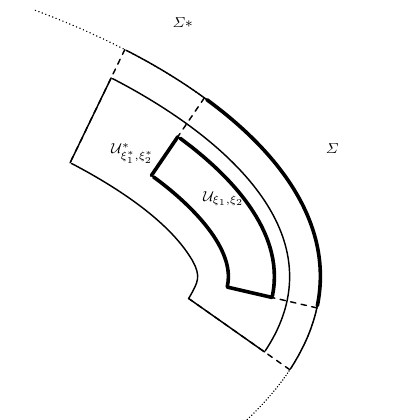
\includegraphics[width=0.48\textwidth]{figures/fig-iv-1-boundary-neighborhoods.png}
  \caption{Proposition~\ref{prop:chap4-zero-tangential-gradient-trace} 证明中的记号}
  \label{fig:chap4-boundary-neighborhoods}
 \end{figure}
 按构造, $F$ 的切向部分 $F_T$ 为零. 因此 Proposition~\ref{prop:chap3-divergence-normal-tangential} 给出
 \[
  \operatorname{div}F
  =\nabla_NF_N+\frac{\nabla_NJ}{J}F_N
  =\frac1J\nabla_N(JF_N).
 \]
 按 $F$ 的定义,
 \[
  (JF_N)(x)=J(P(x))g(P(x));
 \]
 即乘积 $JF_N$ 只依赖于 $x$ 在边界上的投影. 由式\eqref{eq:chap3-normal-derivative-parametrized}可知 $\nabla_N(JF_N)=0$, 因而 $\operatorname{div}F=0$.

 按构造, $F$ 在 $\Omega$ 中光滑、无散度, 并在边界 $\partial\Omega$ 上满足 $F\cdot\nu=g$. 此外, 由于 $g$ 支撑于 $\Sigma_0$, 可见 $F$ 支撑于 $U_{0,s_0}$.

 \item 取截断函数 $\beta\in C_c^\infty(]-2s_0/3,2s_0/3[)$, 满足 $\beta=1$ 于 $]-s_0/3,s_0/3[$. 定义 $F^*(x)=\beta(\rho(x))F(x)$. 可见 $F^*$ 仍满足边界条件 $F^*\cdot\nu=g$, 紧支撑于 $U_{0,2s_0/3}$, 并在 $U_{0,s_0/3}^*$ 上满足无散度条件. 遗憾的是, $F^*$ 在整个集合 $U_{0,s_0}^*$ 上不再无散度.

 \item 令 $f^*=\operatorname{div}(F^*)$, 它紧支撑于 $U_{s_0/3,2s_0/3}$, 并满足
 \[
  \int_{U_{s_0/3,2s_0/3}}f^*\,\mathrm dx
  =\int_{\Sigma_{s_0/3}}F^*\cdot\nu\,\mathrm d\sigma
  =\int_\Sigma F^*\cdot\nu\,\mathrm d\sigma
  =\int_\Sigma g\,\mathrm d\sigma=0,
 \]
 因为按构造 $\operatorname{div}F^*$ 在 $U_{0,s_0/3}$ 中为零.

 所以由 Theorem~\ref{thm:chap4-divergence-right-inverse}, 存在 $\Phi^*\in(H_0^1(U_{s_0/3,2s_0/3}))^3$, 使得 $\operatorname{div}\Phi^*=f^*$. 把 $\Phi^*$ 在其定义域外作零延拓, 并令 $F=F^*-\Phi^*$. 则 $F$ 无散度、紧支撑于 $U_{0,2s_0/3}$, 且在 $\Sigma$ 上满足 $F=g\nu$.

 \item 通过在 $\Omega^c$ 中作类似构造, 最终可以假设 $F$ 无散度且紧支撑于 $U_{-2s_0/3,2s_0/3}$. 引入磨光核 $\eta\in C_c^\infty(B(0,1))$, 并令 $\eta_\varepsilon=\varepsilon^{-3}\eta(\cdot/\varepsilon)$, 再定义
 \[
  F_\varepsilon=F*\eta_\varepsilon.
 \]
 当 $\varepsilon$ 足够小时, $F_\varepsilon$ 光滑、无散度且紧支撑于 $U_{-s_0,s_0}^*$.

 可以假设 $\Sigma_0$ 和 $s_0$ 足够小, 使 $U_{-s_0,s_0}^*$ 是星形的, 因为 $\partial\Omega$ 足够光滑. 因而由 Lemma~\ref{lem:chap4-poincare-compact-vector-potential}, 存在 $\Psi_\varepsilon\in(C_c^\infty(U_{-s_0,s_0}^*))^3$, 使得 $F_\varepsilon=\operatorname{curl}\Psi_\varepsilon$.

 \item 把 $\Psi_\varepsilon$ 在整个空间 $\mathbb R^3$ 上作零延拓, 并在式\eqref{eq:chap4-gradient-curl-orthogonality}中用它作为测试函数, 得到
 \[
  \begin{aligned}
  0
  &=\int_\Omega\nabla p\cdot\operatorname{curl}\Psi_\varepsilon\,\mathrm dx
   =\int_\Omega\nabla p\cdot F_\varepsilon\,\mathrm dx\\
  &=-\int_\Omega p\operatorname{div}(F_\varepsilon)\,\mathrm dx
   +\int_{\Sigma^*}\gamma_0(p)F_\varepsilon\cdot\nu\,\mathrm d\sigma.
  \end{aligned}
 \]
 由于 $F_\varepsilon$ 在 $\Sigma^*$ 的邻域中光滑, 可在这个公式中令 $\varepsilon\to0$, 得到
 \[
  0=\int_\Sigma\gamma_0(p)F\cdot\nu\,\mathrm d\sigma
  =\int_\Sigma\gamma_0(p)g\,\mathrm d\sigma.
 \]
 对 $\Sigma$ 上任意均值为零的 $g$ 都成立这一性质, 因而如预期地推出 $\gamma_0(p)$ 在 $\Sigma$ 上为常数.
\end{itemize}
\end{Proof}

现在定义空间
\[
 \begin{aligned}
 H_{\operatorname{div},\operatorname{curl},\nu}(\Omega)
 =\{u\in(L^2(\Omega))^3:
 &\ \operatorname{div}u\in L^2(\Omega),\\
 &\ \operatorname{curl}u\in(L^2(\Omega))^3,
 \ \gamma_\nu(u)\in H^{1/2}(\partial\Omega)\},
 \end{aligned}
\]
并赋予范数
\[
 \|u\|_{H_{\operatorname{div},\operatorname{curl},\nu}}
 =\bigl(\|u\|_{L^2}^2+\|\operatorname{div}u\|_{L^2}^2
 +\|\operatorname{curl}u\|_{L^2}^2
 +\|\gamma_\nu(u)\|_{H^{1/2}}^2\bigr)^{1/2}.
\]
还定义 $H_{\operatorname{div},\operatorname{curl},\nu}(\Omega)$ 的如下闭子空间:
\begin{equation}
 H_{\operatorname{div},\operatorname{curl},\nu,0}(\Omega)
 =\{u\in H_{\operatorname{div},\operatorname{curl},\nu}(\Omega),\ \gamma_\nu(u)=0\}.
 \label{eq:chap4-hdivcurlnu-zero-space}
\end{equation}

\begin{Lemma}
\label{lem:chap4-divcurl-zero-kernel}
设 $\Omega$ 是 $\mathbb R^3$ 中单连通的 Lipschitz 区域. 若 $u\in(L^2(\Omega))^3$ 满足
\[
 \operatorname{div}u=0,\qquad
 \operatorname{curl}u=0,\qquad
 \gamma_\nu(u)=0,
\]
则 $u=0$.
\end{Lemma}

\begin{Proof}
由假设 $u\in H_{\operatorname{div}}(\Omega)$, 所以迹 $\gamma_\nu(u)$ 必须按 $H^{-1/2}(\partial\Omega)$ 的意义理解.

任取球 $B\subset\Omega$. 设 $\Phi\in(C_c^\infty(B))^3$ 且 $\operatorname{div}\Phi=0$. 由 Lemma~\ref{lem:chap4-poincare-compact-vector-potential}, 存在 $\Psi\in(C_c^\infty(B))^3$, 使得 $\operatorname{curl}\Psi=\Phi$. 因而
\[
 \langle u,\Phi\rangle_{H^{-1}(B),H_0^1(B)}
 =\int_Bu\cdot\Phi\,\mathrm dx
 =\int_Bu\cdot\operatorname{curl}\Psi\,\mathrm dx.
\]
使用 Stokes 公式\eqref{eq:chap4-hcurl-stokes-formula}, 得到
\[
 \langle u,\Phi\rangle_{H^{-1}(B),H_0^1(B)}
 =\int_B(\operatorname{curl}u)\cdot\Psi\,\mathrm dx
 +\langle\gamma_{\wedge\nu}(u),\Psi\rangle_{H^{-1/2},H^{1/2}}.
\]
由于 $\operatorname{curl}u=0$ 且 $\Psi$ 紧支撑于 $B$, 对任意这样的 $\Phi$ 有 $\langle u,\Phi\rangle_{H^{-1},H_0^1}=0$.

由 Theorem~\ref{thm:chap4-de-rham}, 存在 $p_B\in L_0^2(B)$, 使 $u=\nabla p_B$ 于 $B$. 事实上 $p_B\in H^1(B)$, 因为 $u\in(L^2(B))^3$.

此外, $\Delta p_B=\operatorname{div}(\nabla p_B)=\operatorname{div}u=0$, 这意味着 $p_B$ 在 $B$ 中调和, 因而 $p_B\in C^\infty(B)$ (例如见\MBUnresolvedReference{bib:harmonic-smoothness}{[56]}). 最终 $u=\nabla p_B$ 也属于 $(C^\infty(B))^3$. 由于对 $\Omega$ 中任意球 $B$ 都成立, 最终已经证明 $u\in(C^\infty(\Omega))^3$.

现在应用 Lemma~\ref{lem:chap4-poincare-simply-connected}, 得到存在 $p\in C^\infty(\Omega)$, 使 $u=\nabla p$ 于 $\Omega$. 此外, $p$ 是调和函数.

注意 $\nabla p\in(L^2(\Omega))^3$ 且 $p\in L_{\mathrm{loc}}^2(\Omega)$. 所以对任意满足 $\operatorname{div}\Phi=0$ 的 $\Phi\in(C_c^\infty(\Omega))^3$, 有
\[
 \langle u,\Phi\rangle_{H^{-1},H_0^1}
 =\int_\Omega u\cdot\Phi\,\mathrm dx
 =\int_\Omega\nabla p\cdot\Phi\,\mathrm dx
 =-\langle p,\operatorname{div}\Phi\rangle_{\mathcal D',\mathcal D}=0.
\]
由 Theorem~\ref{thm:chap4-de-rham}, 推出存在 $q\in L_0^2(\Omega)$, 使 $u=\nabla q$. 由于 $\Omega$ 连通, $p-q$ 为常数, 因而 $p\in L^2(\Omega)$. 最终 $u=\nabla p$, 其中 $p\in H^1(\Omega)$.

最后应用 Stokes 公式\eqref{eq:chap4-hdiv-stokes-formula}:
\[
 \begin{aligned}
 \int_\Omega|\nabla p|^2\,\mathrm dx
 &=\int_\Omega u\cdot\nabla p\,\mathrm dx\\
 &=-\int_\Omega(\operatorname{div}u)p\,\mathrm dx
 +\langle\gamma_\nu(u),\gamma_0(p)\rangle_{H^{-1/2},H^{1/2}}.
 \end{aligned}
\]
右端两项都为零, 因为 $\operatorname{div}u=0$ 且 $\gamma_\nu(u)=0$. 因而 $u=\nabla p=0$, 结论得证.
\end{Proof}
\paragraph{稠密性结果及其应用}

我们将证明, 空间 $H_{\operatorname{div},\operatorname{curl},\nu}(\Omega)$ 和
$H_{\operatorname{div},\operatorname{curl},\nu,0}(\Omega)$ 分别在代数意义和拓扑意义下等于
$(H^1(\Omega))^3$ 和 $(H^1(\Omega))^3\cap\operatorname{Ker}\gamma_\nu$.

为此, 首先需要下面的稠密性结果.

\begin{Theorem}
\label{thm:chap4-density-hdivcurlnu}
设 $\Omega$ 是 $C^{1,1}$ 类有界连通区域. 集合
\[
 \mathcal H=\left\{u\in(C^{0,1}(\overline\Omega))^3\cap(C^\infty(\Omega))^3,
 \ u\cdot\nu=0\text{ in a neighborhood of }\partial\Omega\right\}
\]
在 $H_{\operatorname{div},\operatorname{curl},\nu,0}(\Omega)$ 中稠密, 也在
$(H^1(\Omega))^3\cap\operatorname{Ker}\gamma_\nu$ 中稠密.
\end{Theorem}

\begin{Proof}
\begin{enumerate}
 \item 首先证明 $\mathcal H$ 在 $(H^1(\Omega))^3\cap\operatorname{Ker}\gamma_\nu$ 中稠密. 设
 $v\in(H^1(\Omega))^3$ 且 $\gamma_\nu(v)=0$ 于 $\partial\Omega$. 设
 $\mathcal O_{s_0}^{\rho}$ 是 $\partial\Omega$ 的一个邻域, 在其中可以使用切向和法向坐标
 (见 Chapter~\ref{chap:sobolev-spaces} 的 Section~\ref{sec:chap3-boundary-calculus}), 并取
 $\varphi\in C_c^\infty(\overline\Omega)$, 使得
 $\operatorname{Supp}(1-\varphi)\subset\mathcal O_{s_0}^{\rho}$.

 写成 $v=\varphi v+(1-\varphi)v$. 按构造, $\varphi v\in(H_0^1(\Omega))^3$, 因而可以由
 $(\mathcal D(\Omega))^3\subset\mathcal H$ 中的函数序列在 $H^1$ 范数下逼近. 只需处理
 $u=(1-\varphi)v$. 由于 $u$ 支撑于 $\mathcal O_{s_0}^{\rho}$, 可以定义其切向部分
 $u_T=u-(u\cdot\nu)\nu$; 它与 $u$ 具有相同正则性 (因为 $\nu$ 是 Lipschitz 连续的), 并满足
 $u_T\cdot\nu=0$ 于 $\mathcal O_{s_0}^{\rho}$. 由于 $\varphi=0$ 于 $\partial\Omega$, 有
 \[
  u\cdot\nu=v\cdot\nu=0,\qquad\text{on }\partial\Omega.
 \]
 因而 $u\cdot\nu\in H_0^1(\mathcal O_{s_0}^{\rho})$ 且
 $u_T\in(H^1(\mathcal O_{s_0}^{\rho}))^3$. 所以对任意 $\varepsilon>0$, 可以找到
 $u_{T,\varepsilon}\in(C^\infty(\overline{\mathcal O_{s_0}^{\rho}}))^3$ 和
 $f_\varepsilon\in\mathcal D(\mathcal O_{s_0}^{\rho})$, 使得
 \[
  \|f_\varepsilon-(u\cdot\nu)\|_{H^1(\mathcal O_{s_0}^{\rho})}
  +\|u_{T,\varepsilon}-u_T\|_{H^1(\mathcal O_{s_0}^{\rho})}
  \underset{\varepsilon\to0}{\longrightarrow}0.
 \]
 令
 \[
  u_\varepsilon=u_{T,\varepsilon}-(u_{T,\varepsilon}\cdot\nu)\nu+f_\varepsilon\nu.
 \]
 注意到 $u_\varepsilon\cdot\nu=f_\varepsilon$ 于 $\mathcal O_{s_0}^{\rho}$, 所以
 $u_\varepsilon\cdot\nu$ 在边界的一个邻域中恒为零. 由于 $\nu$ 在 $\overline\Omega$ 上 Lipschitz 连续,
 且在 $\mathcal O_{s_0}^{\rho}$ 中属于 $C^\infty$ 类, 可见 $u_\varepsilon$ 具有所需的正则性.
 此外, 按构造 $u_T\cdot\nu=0$, 因而
 \[
  \begin{aligned}
  \|u-u_\varepsilon\|_{H^1}
  &=\|u_{T,\varepsilon}-u_T-((u_{T,\varepsilon}-u_T)\cdot\nu)\nu
    +(\psi_\varepsilon-(u\cdot\nu))\nu\|_{H^1}\\
  &\leq C\|u_{T,\varepsilon}-u_T\|_{H^1}
    +C\|\psi_\varepsilon-(u\cdot\nu)\|_{H^1}
    \underset{\varepsilon\to0}{\longrightarrow}0,
  \end{aligned}
 \]
 这证明了结果的第一部分.

 \item 现在处理第二个稠密性结果. 设
 $v\in H_{\operatorname{div},\operatorname{curl},\nu,0}(\Omega)$, 并对任意 $\varepsilon>0$ 定义
 $\widetilde v_\varepsilon=S_\varepsilon v\in(C^\infty(\overline\Omega))^3$, 其中
 $(S_\varepsilon)_\varepsilon$ 是 Chapter~\ref{chap:sobolev-spaces} 的
 Section~\ref{subsec:chap3-mollifiers-friedrichs} 中定义的磨光算子族.

 由 Theorem~\ref{thm:chap3-graph-space-density}, 有
 \[
  \widetilde v_\varepsilon\to v\text{ in }L^2(\Omega),\qquad
  \operatorname{div}\widetilde v_\varepsilon\to\operatorname{div}v\text{ in }L^2(\Omega),
 \]
 以及
 \[
  \operatorname{curl}\widetilde v_\varepsilon\to\operatorname{curl}v
  \text{ in }(L^2(\Omega))^3.
 \]
 注意 $\widetilde v_\varepsilon\cdot\nu$ 在 $\partial\Omega$ 上未必为零. 现在考虑 Neumann 问题
 \[
 \left\{
 \begin{aligned}
 -\Delta f_\varepsilon
 &=\frac1{|\Omega|}\int_{\partial\Omega}\widetilde v_\varepsilon\cdot\nu\,\mathrm d\sigma
 =\frac1{|\Omega|}\langle\gamma_\nu(\widetilde v_\varepsilon),1\rangle_{H^{-1/2},H^{1/2}}
 &&\text{in }\Omega,\\
 -\frac{\partial f_\varepsilon}{\partial\nu}
 &=\widetilde v_\varepsilon\cdot\nu&&\text{on }\partial\Omega,\\
 \int_\Omega f_\varepsilon\,\mathrm dx&=0.
 \end{aligned}
 \right.
 \]
 首先, 因为 $\widetilde v_\varepsilon$ 光滑且 $\nu$ 是 Lipschitz 向量场,
 $\widetilde v_\varepsilon\cdot\nu$ 是 Lipschitz 连续的, 故属于 $H^{1/2}(\partial\Omega)$.
 该 Neumann 问题的源项为常值函数, 因而相容条件成立; 由
 Theorem~\ref{thm:chap3-laplace-neumann} 可知 $f_\varepsilon\in H^2(\Omega)$,
 因为假设 $\Omega$ 属于 $C^{1,1}$ 类.

 其次, 由迹算子 $\gamma_\nu$ 的连续性及 $\gamma_\nu(v)=0$, 有
 \[
  \|\widetilde v_\varepsilon\cdot\nu\|_{H^{-1/2}}
  =\|\gamma_\nu(\widetilde v_\varepsilon-v)\|_{H^{-1/2}}
  \leq C\bigl(\|v-\widetilde v_\varepsilon\|_{L^2}
  +\|\operatorname{div}v-\operatorname{div}\widetilde v_\varepsilon\|_{L^2}\bigr),
 \]
 因而 $\widetilde v_\varepsilon\cdot\nu\to0$ 于 $H^{-1/2}(\partial\Omega)$.
 Laplace--Neumann 问题的能量估计\eqref{eq:chap3-neumann-energy-bound}给出
 \[
  \|\nabla f_\varepsilon\|_{L^2}
  \leq C\|\widetilde v_\varepsilon\cdot\nu\|_{H^{-1/2}}
  \underset{\varepsilon\to0}{\longrightarrow}0.
 \]
 此外, 按构造
 \[
  \|\Delta f_\varepsilon\|_{L^2}
  =C_\Omega\left|\int_{\partial\Omega}\widetilde v_\varepsilon\cdot\nu\,\mathrm d\sigma\right|
  \underset{\varepsilon\to0}{\longrightarrow}0.
 \]

 现在定义 $v_\varepsilon=\widetilde v_\varepsilon+\nabla f_\varepsilon$;
 它属于 $(H^1(\Omega))^3$, 并满足
 \[
  \|v_\varepsilon-v\|_{L^2}
  \leq\|\widetilde v_\varepsilon-v\|_{L^2}+\|\nabla f_\varepsilon\|_{L^2}
  \underset{\varepsilon\to0}{\longrightarrow}0,
 \]
 \[
  \|\operatorname{div}v_\varepsilon-\operatorname{div}v\|_{L^2}
  \leq\|\operatorname{div}\widetilde v_\varepsilon-\operatorname{div}v\|_{L^2}
  +\|\Delta f_\varepsilon\|_{L^2}
  \underset{\varepsilon\to0}{\longrightarrow}0,
 \]
 并且由于 $\operatorname{curl}\nabla f_\varepsilon=0$,
 \[
  \|\operatorname{curl}v_\varepsilon-\operatorname{curl}v\|_{L^2}
  =\|\operatorname{curl}\widetilde v_\varepsilon-\operatorname{curl}v\|_{L^2}
  \underset{\varepsilon\to0}{\longrightarrow}0.
 \]
 总之, 我们证明了 $v_\varepsilon\in(H^1(\Omega))^3\cap\operatorname{Ker}\gamma_\nu$, 且
 \begin{equation}
  \|v_\varepsilon-v\|_{H_{\operatorname{div},\operatorname{curl},\nu}}
  \underset{\varepsilon\to0}{\longrightarrow}0.
  \label{eq:chap4-density-first-convergence}
 \end{equation}
 现在使用上面已证明的 $\mathcal H$ 在 $(H^1(\Omega))^3\cap\operatorname{Ker}\gamma_\nu$ 中的稠密性.
 可以找到 $w_\varepsilon\in\mathcal H$, 使得
 $\|v_\varepsilon-w_\varepsilon\|_{H^1}\to0$. 但由于
 $v_\varepsilon,w_\varepsilon\in(H^1(\Omega))^3$, 显然有
 \begin{equation}
  \|v_\varepsilon-w_\varepsilon\|_{H_{\operatorname{div},\operatorname{curl},\nu}}
  \leq C\|v_\varepsilon-w_\varepsilon\|_{H^1}
  \underset{\varepsilon\to0}{\longrightarrow}0.
  \label{eq:chap4-density-second-convergence}
 \end{equation}
 由式\eqref{eq:chap4-density-first-convergence}和\eqref{eq:chap4-density-second-convergence},
 推出 $w_\varepsilon\in\mathcal H$ 在 $H_{\operatorname{div},\operatorname{curl},\nu}(\Omega)$ 中收敛到 $v$, 结论得证.
\end{enumerate}
\end{Proof}

\begin{Theorem}
\label{thm:chap4-hdivcurlnu-equals-h1}
设 $\Omega$ 是 $\mathbb R^3$ 中 $C^{1,1}$ 类有界区域. 成立等式
\begin{align}
 H_{\operatorname{div},\operatorname{curl},\nu,0}(\Omega)
 &=(H^1(\Omega))^3\cap\operatorname{Ker}\gamma_\nu,
 \label{eq:chap4-hdivcurlnu-zero-equals-h1}\\
 H_{\operatorname{div},\operatorname{curl},\nu}(\Omega)
 &=(H^1(\Omega))^3,
 \label{eq:chap4-hdivcurlnu-equals-h1}
\end{align}
并且存在仅依赖于 $\Omega$ 的 $C>0$, 使得
\begin{equation}
 \|u\|_{H^1}\leq C\bigl(
 \|u\|_{L^2}+\|\operatorname{div}u\|_{L^2}
 +\|\operatorname{curl}u\|_{L^2}+\|\gamma_\nu(u)\|_{H^{1/2}}\bigr),
 \label{eq:chap4-hdivcurlnu-h1-estimate}
\end{equation}
对任意 $u\in(H^1(\Omega))^3=H_{\operatorname{div},\operatorname{curl},\nu}(\Omega)$ 成立.
也就是说, $H^1$ 范数与 $H_{\operatorname{div},\operatorname{curl},\nu}$ 范数在
$(H^1(\Omega))^3$ 中等价.

此外, 若 $\Omega$ 单连通, 则式\eqref{eq:chap4-hdivcurlnu-h1-estimate}可替换为
\begin{equation}
 \|u\|_{H^1}\leq C\bigl(
 \|\operatorname{div}u\|_{L^2}+\|\operatorname{curl}u\|_{L^2}
 +\|\gamma_\nu(u)\|_{H^{1/2}}\bigr),
 \label{eq:chap4-hdivcurlnu-poincare-estimate}
\end{equation}
对任意 $u\in(H^1(\Omega))^3=H_{\operatorname{div},\operatorname{curl},\nu}(\Omega)$ 成立.
\end{Theorem}

\begin{Proof}
\begin{itemize}
 \item 首先假设式\eqref{eq:chap4-hdivcurlnu-h1-estimate}对任意向量场
 $u\in(H^1(\Omega))^3$ 成立; 我们证明等式\eqref{eq:chap4-hdivcurlnu-zero-equals-h1}成立.

 考虑从 $(H^1(\Omega))^3\cap\operatorname{Ker}\gamma_\nu$ 到
 $H_{\operatorname{div},\operatorname{curl},\nu,0}(\Omega)$ 的恒等映射 $I$.
 \begin{itemize}
  \item 按 $H_{\operatorname{div},\operatorname{curl},\nu}$ 范数的定义, 显然 $I$ 连续.
  \item $I$ 的像在 $H_{\operatorname{div},\operatorname{curl},\nu,0}(\Omega)$ 中闭.
  事实上, 若 $(u_n)_n$ 是 $(H^1(\Omega))^3\cap\operatorname{Ker}\gamma_\nu$ 中的序列,
  且在 $H_{\operatorname{div},\operatorname{curl},\nu,0}(\Omega)$ 中收敛, 则由
  式\eqref{eq:chap4-hdivcurlnu-h1-estimate}, $(u_n)_n$ 是 $(H^1(\Omega))^3$ 中的 Cauchy 序列;
  所以它收敛到某个 $u\in(H^1(\Omega))^3\cap\operatorname{Ker}\gamma_\nu$, 且显然该函数 $u$ 也是
  $(u_n)_n$ 在 $H_{\operatorname{div},\operatorname{curl},\nu,0}(\Omega)$ 中的极限.
  \item 由 Theorem~\ref{thm:chap4-density-hdivcurlnu}, 知道包含于 $I$ 的像中的空间
  $\mathcal H$ 在 $H_{\operatorname{div},\operatorname{curl},\nu,0}(\Omega)$ 中稠密;
  因而 $I$ 的像在该空间中稠密.
 \end{itemize}
 最终, $I$ 的像在 $H_{\operatorname{div},\operatorname{curl},\nu,0}(\Omega)$ 中既闭又稠密,
 所以其像就是整个空间, 这证明了式\eqref{eq:chap4-hdivcurlnu-zero-equals-h1}.

 随后推出式\eqref{eq:chap4-hdivcurlnu-equals-h1}. 事实上, 对任意
 $u\in H_{\operatorname{div},\operatorname{curl},\nu}(\Omega)$, 因为
 $\gamma_\nu(u)\in H^{1/2}(\partial\Omega)$, 可以使用提升算子 $R_0$, 令
 \[
  v=u-R_0(\gamma_\nu(u)\nu).
 \]
 由于 $R_0(\gamma_\nu(u)\nu)\in(H^1(\Omega))^3$, 按构造可知
 $v\in H_{\operatorname{div},\operatorname{curl},\nu,0}(\Omega)$.
 由式\eqref{eq:chap4-hdivcurlnu-zero-equals-h1}, 推出 $v\in(H^1(\Omega))^3$,
 进而 $u=v+R_0(\gamma_\nu(u)\nu)$ 也属于 $(H^1(\Omega))^3$.

 \item 还需对任意 $u\in(H^1(\Omega))^3$ 证明式\eqref{eq:chap4-hdivcurlnu-h1-estimate}.
 首先, 与上面相同地使用提升算子 $R_0$, 可见只需对
 $u\in(H^1(\Omega))^3\cap\operatorname{Ker}\gamma_\nu$ 证明该不等式.

 由 Theorem~\ref{thm:chap4-density-hdivcurlnu}, 可以找到序列 $\varphi_n\in\mathcal H$,
 它在 $(H^1(\Omega))^3$ 中收敛到 $u$. 因而, 如果能够对所有 $\varphi\in\mathcal H$
 证明式\eqref{eq:chap4-hdivcurlnu-h1-estimate}, 结果便由稠密性得到.

 设 $\varphi\in\mathcal H$. 由公式\MBUnresolvedReference{eq:appendix-vector-laplacian}{(A.9)}, 有
 $-\Delta\varphi\cdot\varphi
 =\operatorname{curl}\operatorname{curl}\varphi\cdot\varphi
 -\nabla(\operatorname{div}\varphi)\cdot\varphi$.
 在 $\Omega$ 上积分并对各项使用 Stokes 公式, 得到
 \begin{equation}
 \begin{aligned}
 \int_\Omega|\nabla\varphi|^2\,\mathrm dx
 ={}&\int_\Omega\bigl(|\operatorname{curl}\varphi|^2
 +|\operatorname{div}\varphi|^2\bigr)\,\mathrm dx\\
 &+\int_{\partial\Omega}\bigl((\varphi\wedge\nu)\cdot(\operatorname{curl}\varphi)
 +(\nu\cdot\nabla)\varphi\cdot\varphi
 -(\operatorname{div}\varphi)(\varphi\cdot\nu)\bigr)\,\mathrm d\sigma.
 \end{aligned}
 \label{eq:chap4-gradient-curl-div-boundary}
 \end{equation}
 使用公式\MBUnresolvedReference{eq:appendix-vector-a3}{(A.3)},
 \MBUnresolvedReference{eq:appendix-vector-a4}{(A.4)},
 \MBUnresolvedReference{eq:appendix-vector-a7}{(A.7)}和
 \MBUnresolvedReference{eq:appendix-vector-a8}{(A.8)}, 可以写成
 \[
 \begin{aligned}
 &(\varphi\wedge\nu)\cdot(\operatorname{curl}\varphi)
 +(\nu\cdot\nabla)\varphi\cdot\varphi\\
 &\quad=\operatorname{div}(\varphi\wedge(\varphi\wedge\nu))
 +\varphi\cdot\operatorname{curl}(\varphi\wedge\nu)
 +(\nu\cdot\nabla)\frac{|\varphi|^2}{2}\\
 &\quad=\operatorname{div}((\varphi\cdot\nu)\varphi-|\varphi|^2\nu)
 +(\nu\cdot\nabla)\frac{|\varphi|^2}{2}\\
 &\qquad+\varphi\cdot\bigl((\operatorname{div}\nu)\varphi
 -(\operatorname{div}\varphi)\nu+(\nu\cdot\nabla)\varphi-(\varphi\cdot\nabla)\nu\bigr)\\
 &\quad=(\varphi\cdot\nabla)(\varphi\cdot\nu)-((\varphi\cdot\nabla)\nu)\cdot\varphi\\
 &\quad=((\varphi\cdot\nabla)\varphi)\cdot\nu.
 \end{aligned}
 \]
 因而边界项可以写成
 \[
 \begin{aligned}
 &(\varphi\wedge\nu)\cdot(\operatorname{curl}\varphi)
 +(\nu\cdot\nabla)\varphi\cdot\varphi
 -(\operatorname{div}\varphi)(\varphi\cdot\nu)\\
 &\quad=((\varphi\cdot\nabla)\varphi)\cdot\nu-(\operatorname{div}\varphi)(\varphi\cdot\nu)\\
 &\quad=-((\varphi\cdot\nabla)\nu)\cdot\varphi
 +(\varphi\cdot\nabla)(\varphi\cdot\nu)
 -(\operatorname{div}\varphi)(\varphi\cdot\nu).
 \end{aligned}
 \]
 因为 $\varphi\in\mathcal H$, 知道 $\varphi\cdot\nu=0$ 于边界的一个邻域.
 所以上式最后两项消失, 由式\eqref{eq:chap4-gradient-curl-div-boundary}最终得到
 \begin{equation}
 \int_\Omega|\nabla\varphi|^2\,\mathrm dx
 =\int_\Omega\bigl(|\operatorname{curl}\varphi|^2+|\operatorname{div}\varphi|^2\bigr)\,\mathrm dx
 -\int_{\partial\Omega}((\varphi\cdot\nabla)\nu)\cdot\varphi\,\mathrm d\sigma.
 \label{eq:chap4-gradient-curl-div-identity}
 \end{equation}
 记该等式最后一项为 $I$; 它不含 $\varphi$ 的任何导数, 所以
 \[
  |I|\leq\operatorname{Lip}(\nu)\|\varphi\|_{L^2(\partial\Omega)}^2.
 \]
 由 Theorem~\ref{thm:chap3-boundary-sobolev-embedding} 中的迹不等式,
 \[
  \|\varphi\|_{L^2(\partial\Omega)}
  \leq C\|\varphi\|_{L^2}+C\|\varphi\|_{L^2}^{1/2}\|\nabla\varphi\|_{L^2}^{1/2}.
 \]
 再使用 Young 不等式 (见 Corollary~\ref{cor:chap2-young-epsilon}), 得到
 \[
  |I|\leq C_\varepsilon\|\varphi\|_{L^2}^2
  +\frac12\|\nabla\varphi\|_{L^2}^2.
 \]
 将这个估计用于式\eqref{eq:chap4-gradient-curl-div-identity}, 即得所需结论.

 \item 现在假设 $\Omega$ 单连通, 并仿照 Poincaré 不等式的证明
 (见 Propositions~\ref{prop:chap3-generalized-poincare}和
 \ref{prop:chap3-poincare-wirtinger}), 用反证法证明
 式\eqref{eq:chap4-hdivcurlnu-poincare-estimate}.

 假设式\eqref{eq:chap4-hdivcurlnu-poincare-estimate}不成立, 则存在序列
 $(u_n)_n\in(H^1(\Omega))^3$, 使得
 \begin{equation}
  \|u_n\|_{H^1}=1,\qquad\forall n\geq0,
  \label{eq:chap4-contradiction-unit-norm}
 \end{equation}
 以及
 \begin{equation}
  \|\operatorname{div}u_n\|_{L^2}+\|\operatorname{curl}u_n\|_{L^2}
  +\|\gamma_\nu(u_n)\|_{H^{1/2}}
  \underset{n\to+\infty}{\longrightarrow}0.
  \label{eq:chap4-contradiction-data-zero}
 \end{equation}
 因为 $\Omega$ 有界, $H^1(\Omega)$ 到 $L^2(\Omega)$ 的嵌入是紧的;
 因而存在子序列 (仍记为 $(u_n)_n$), 它在 $(L^2(\Omega))^3$ 中强收敛到某个
 $u\in(H^1(\Omega))^3$. 由式\eqref{eq:chap4-contradiction-data-zero}, 极限满足
 $\operatorname{div}u=0$, $\operatorname{curl}u=0$ 且 $\gamma_\nu(u)=0$.
 利用 $\Omega$ 单连通的假设, Lemma~\ref{lem:chap4-divcurl-zero-kernel} 给出 $u=0$.
 所以除了式\eqref{eq:chap4-contradiction-data-zero}之外, 必有
 $\|u_n\|_{L^2}\to0$. 再由式\eqref{eq:chap4-hdivcurlnu-h1-estimate}, 推出
 $\|u_n\|_{H^1}\to0$, 这与式\eqref{eq:chap4-contradiction-unit-norm}矛盾.
\end{itemize}
\end{Proof}

同类结果对更高正则性的 Sobolev 空间也成立. 为简单起见, 我们只陈述对应于 $H^2$ 正则性的结果.

\begin{Theorem}
\label{thm:chap4-hdivcurl-h2-regularity}
设 $\Omega$ 是 $\mathbb R^3$ 中 $C^{2,1}$ 类有界区域. 对任意满足
\[
u\in(H^1(\Omega))^3,\qquad
\operatorname{div}u\in H^1(\Omega),\qquad
\operatorname{curl}u\in(H^1(\Omega))^3,\qquad
 \gamma_\nu(u)\in H^{3/2}(\partial\Omega)
\]
的 $u$, 有 $u\in(H^2(\Omega))^3$, 且
\[
 \|u\|_{H^2}\leq C\bigl(\|u\|_{L^2}+\|\operatorname{div}u\|_{H^1}
 +\|\operatorname{curl}u\|_{H^1}+\|\gamma_\nu(u)\|_{H^{3/2}}\bigr),
\]
其中 $C>0$ 仅依赖于 $\Omega$.
\end{Theorem}

该 Theorem 的证明在 Section~\MBUnresolvedReference{sec:chap4-stokes-higher-regularity}{6.4} 中给出,
因为需要使用稍后研究 Stokes 问题正则性时引入的一些工具.

\subsubsection{旋度算子的核与像}
\label{subsec:chap4-curl-kernel-image}

\begin{Lemma}
\label{lem:chap4-curl-kernel-gradients}
设 $\Omega$ 是 $\mathbb R^3$ 中 $C^{1,1}$ 类单连通区域. 对任意满足
$\operatorname{curl}u=0$ 的 $u\in(L^2(\Omega))^3$, 存在 $p\in H^1(\Omega)$, 使得
$u=\nabla p$. 换言之,
\[
 \operatorname{Ker}_{L^2}(\operatorname{curl})=\nabla(H^1(\Omega)).
\]
\end{Lemma}

\begin{Proof}
将这样的 $u$ 作 Leray 分解 (Definition~\ref{def:chap4-leray-decomposition}):
\[
 u=u_0+\nabla p,
\]
其中 $p\in H^1(\Omega)$, $\operatorname{div}u_0=0$ 且 $\gamma_\nu(u_0)=0$.
对该公式取旋度得到 $\operatorname{curl}u=\operatorname{curl}u_0=0$.
因而由 Lemma~\ref{lem:chap4-divcurl-zero-kernel}, 有 $u_0=0$, 从而 $u=\nabla p$.
\end{Proof}

\refstepcounter{chapterfoursectionfourremark}
\paragraph{Remark~\thechapterfoursectionfourremark.}\label{rem:chap4-curl-kernel-neumann-regularity}
我们强调, 对于 $\operatorname{Ker}_{L^2}(\operatorname{curl})=\nabla(H^1(\Omega))$ 中的元素,
不等式\eqref{eq:chap4-hdivcurlnu-poincare-estimate}因此写成
\[
 \|\nabla p\|_{H^1}\leq C\left(
 \|\Delta p\|_{L^2}+\left\|\frac{\partial p}{\partial\nu}\right\|_{H^{1/2}}
 \right),
\]
对满足 $\Delta p\in L^2(\Omega)$ 且
$\partial p/\partial\nu\in H^{1/2}(\partial\Omega)$ 的任意 $p\in H^1(\Omega)$ 成立.
注意到这个结果恰好就是具有 Neumann 边界条件的 Laplace 方程的椭圆正则性定理
(见 Theorem~\ref{thm:chap3-laplace-neumann}).

现在可以刻画旋度算子的像.

\begin{Theorem}
\label{thm:chap4-curl-image-characterization}
设 $\Omega$ 是 $\mathbb R^3$ 中 $C^{1,1}$ 类单连通有界区域. 以
$\Gamma_1,\ldots,\Gamma_m$ 表示边界 $\partial\Omega$ 的连通分支.
\begin{enumerate}
 \item 有
 \begin{equation}
  \operatorname{curl}\bigl((H^1(\Omega))^3\bigr)
  =\operatorname{curl}\bigl((H^1(\Omega))^3\cap H\bigr).
  \label{eq:chap4-curl-image-leray-space}
 \end{equation}
 此外, 该空间在 $(L^2(\Omega))^3$ 中闭.

 \item 在 $(L^2(\Omega))^3$ 中有
 \begin{equation}
 \begin{aligned}
 \Bigl(\operatorname{curl}\bigl((H^1(\Omega))^3\bigr)\Bigr)^\perp
 &=\{u\in(L^2(\Omega))^3,\ \operatorname{curl}u=0,\\
 &\hspace{8em}\gamma_{\wedge\nu}(u)=0\}\\
 &=\{u\in(L^2(\Omega))^3,\ u=\nabla p,\ p\in H^1(\Omega),\\
 &\hspace{8em}\gamma_0(p)\text{ is constant on each }\Gamma_i\}.
 \end{aligned}
 \label{eq:chap4-curl-image-orthogonal}
 \end{equation}

 \item 最后有
 \[
  \operatorname{curl}\bigl((H^1(\Omega))^3\bigr)
  =\left\{u\in(L^2(\Omega))^3,
  \ \operatorname{div}u=0,\ \text{satisfying \eqref{eq:chap4-curl-flux-compatibility}}\right\},
 \]
 其中引入了下列相容条件:
 \begin{equation}
  \langle\gamma_\nu(u),1\rangle_{H^{-1/2}(\Gamma_i),H^{1/2}(\Gamma_i)}=0,
  \qquad\forall i=1,\ldots,m.
  \label{eq:chap4-curl-flux-compatibility}
 \end{equation}
\end{enumerate}
\end{Theorem}

\begin{Proof}
\begin{enumerate}
 \item 设 $u=\operatorname{curl}\widetilde\Psi$, 其中
 $\widetilde\Psi\in(H^1(\Omega))^3$. 引入 $\Psi=\mathcal P\widetilde\Psi$,
 即 $\widetilde\Psi$ 在 $H$ 上的 Leray 投影, 于是
 $\widetilde\Psi=\Psi+\nabla q$, 其中 $q\in H^1(\Omega)$, 从而
 $\operatorname{curl}\widetilde\Psi=\operatorname{curl}\Psi=u$.
 此外, Leray 投影把 $(H^1(\Omega))^3$ 映入自身
 (见 Proposition~\ref{prop:chap4-leray-projection-h1}), 所以
 $\Psi\in(H^1(\Omega))^3$. 这证明了两个空间相等.

 注意, 由 Lemma~\ref{lem:chap4-divcurl-zero-kernel}, $\Psi$ 是满足
 $\operatorname{curl}\Psi=u$ 的 $(H^1(\Omega))^3\cap H$ 中唯一元素.
 由不等式\eqref{eq:chap4-hdivcurlnu-h1-estimate}, 得到
 \begin{equation}
  \|\Psi\|_{H^1}\leq C\|\operatorname{curl}\Psi\|_{L^2}=C\|u\|_{L^2}.
  \label{eq:chap4-curl-potential-h1-estimate}
 \end{equation}
 因而 $\operatorname{curl}((H^1(\Omega))^3)$ 是闭的. 事实上, 若
 $(u_n)_n$ 是该空间中收敛到 $u\in(L^2(\Omega))^3$ 的序列, 对每个 $u_n$ 关联唯一的
 $\Psi_n\in(H^1(\Omega))^3\cap H$, 使得 $\operatorname{curl}\Psi_n=u_n$.
 由式\eqref{eq:chap4-curl-potential-h1-estimate}, $(\Psi_n)_n$ 是
 $(H^1(\Omega))^3$ 中的 Cauchy 序列, 因而收敛到某个
 $\Psi\in(H^1(\Omega))^3$. 显然极限满足 $u=\operatorname{curl}\Psi$, 结论得证.

 \item 设 $u\in(L^2(\Omega))^3$ 与
 $\operatorname{curl}((H^1(\Omega))^3)$ 正交. 特别地, 对任意
 $\Phi\in(\mathcal D(\Omega))^3$,
 \[
  \langle\operatorname{curl}u,\Phi\rangle_{\mathcal D',\mathcal D}
  =\langle u,\operatorname{curl}\Phi\rangle_{\mathcal D',\mathcal D}=0,
 \]
 因而 $\operatorname{curl}u=0$. 现在对任意 $v\in(H^1(\Omega))^3$ 使用
 式\eqref{eq:chap4-hcurl-stokes-formula}, 得到
 \[
  0=\int_\Omega u\cdot\operatorname{curl}v\,\mathrm dx
  =\int_\Omega v\cdot\operatorname{curl}u\,\mathrm dx
  +\langle\gamma_{\wedge\nu}(u),\gamma_0(v)\rangle_{H^{-1/2},H^{1/2}}.
 \]
 这推出 $\gamma_{\wedge\nu}(u)=0$, 从而证明了所称等式的第一部分.
 由 Lemma~\ref{lem:chap4-curl-kernel-gradients}, 知道 $u=\nabla p$, 其中
 $p\in(H^1(\Omega))^3$. 条件
 $\gamma_{\wedge\nu}(\nabla p)=\gamma_{\wedge\nu}(u)=0$ 与
 Proposition~\ref{prop:chap4-zero-tangential-gradient-trace} 给出结论.

 \item 对任意 $u\in\operatorname{curl}((H^1(\Omega))^3)$, 显然有
 $\operatorname{div}u=0$. 对任意 $i\in\{1,\ldots,m\}$, 取
 $p_i\in H^1(\Omega)$, 使 $p_i=1$ 于 $\Gamma_i$, 且当 $j\neq i$ 时
 $p_i=0$ 于 $\Gamma_j$. 迹提升定理
 (Theorem~\ref{thm:chap3-trace-lifting-operator}) 保证这样的函数存在.
 利用式\eqref{eq:chap4-curl-image-orthogonal}, 条件 $\operatorname{div}u=0$ 和
 Stokes 公式\eqref{eq:chap4-hdiv-stokes-formula}, 得到
 \[
  0=\int_\Omega u\cdot\nabla p_i\,\mathrm dx
  =\langle\gamma_\nu(u),\gamma_0(p_i)\rangle_{H^{-1/2}(\partial\Omega),H^{1/2}(\partial\Omega)}
  =\langle\gamma_\nu(u),1\rangle_{H^{-1/2}(\Gamma_i),H^{1/2}(\Gamma_i)},
 \]
 这证明了条件\eqref{eq:chap4-curl-flux-compatibility}成立.

 反过来, 假设 $u\in(L^2(\Omega))^3$ 满足 $\operatorname{div}u=0$ 及
 条件\eqref{eq:chap4-curl-flux-compatibility}. 要证明 $u$ 属于旋度算子的像.
 该像在 $(L^2(\Omega))^2$ 中闭, 所以只需证明 $u$ 与
 $\bigl(\operatorname{curl}((H^1(\Omega))^3)\bigr)^\perp$ 中任意元素正交;
 见 Remark~\ref{rem:chap4-annihilator-properties}. 因而使用
 式\eqref{eq:chap4-curl-image-orthogonal}, 取 $w=\nabla p$, 其中
 $p\in H^1(\Omega)$, 且 $\gamma_0(p)$ 在每个 $\Gamma_i$ 上为常数 $p_i$.
 再次使用 Stokes 公式\eqref{eq:chap4-hdiv-stokes-formula}, 得到
 \[
 \begin{aligned}
  \int_\Omega u\cdot w\,\mathrm dx
  &=\int_\Omega u\cdot\nabla p\,\mathrm dx\\
  &=-\int_\Omega(\operatorname{div}u)p\,\mathrm dx
  +\sum_{i=1}^m p_i
  \langle\gamma_\nu(u),1\rangle_{H^{-1/2}(\Gamma_i),H^{1/2}(\Gamma_i)}=0.
 \end{aligned}
 \]
 这证明了结论.
\end{enumerate}
\end{Proof}

\subsubsection{散度/旋度问题}
\label{subsec:chap4-div-curl-problem}

利用前面的全部结果, 现在可以研究散度/旋度问题. 我们先研究法向边界条件的情形,
再研究不施加任何边界条件的情形. 注意, 对这个问题还可以考虑其他类型的边界条件
(这尤其在电磁学中有用), 但这里不予讨论.

\begin{Theorem}
\label{thm:chap4-div-curl-normal-boundary}
采用与 Theorem~\ref{thm:chap4-curl-image-characterization} 相同的记号. 假设给定:
\begin{itemize}
 \item 向量场 $u\in(L^2(\Omega))^3$, 满足 $\operatorname{div}u=0$ 及
 条件\eqref{eq:chap4-curl-flux-compatibility}.
 \item 标量场 $v\in L^2(\Omega)$ 和边界数据
 $\Psi_\nu\in H^{1/2}(\partial\Omega)$, 满足相容条件
 \[
  \int_\Omega v\,\mathrm dx=\int_{\partial\Omega}\Psi_\nu\,\mathrm d\sigma.
 \]
\end{itemize}
则问题
\begin{equation}
\left\{
\begin{aligned}
 \operatorname{div}\Psi&=v&&\text{in }\Omega,\\
 \operatorname{curl}\Psi&=u&&\text{in }\Omega,\\
 \Psi\cdot\nu&=\Psi_\nu&&\text{on }\partial\Omega
\end{aligned}
\right.
\label{eq:chap4-div-curl-normal-problem}
\end{equation}
存在唯一解 $\Psi\in(H^1(\Omega))^3$; 此外它满足
\[
 \|\Psi\|_{H^1}\leq C\bigl(
 \|u\|_{L^2}+\|v\|_{L^2}+\|\Psi_\nu\|_{H^{1/2}}\bigr),
\]
其中 $C>0$ 仅依赖于 $\Omega$.

最后, 若 $\Omega$ 属于 $C^{2,1}$ 类,
$u\in(H^1(\Omega))^3$, $v\in H^1(\Omega)$ 且
$\Psi_\nu\in H^{3/2}(\partial\Omega)$, 则问题
\eqref{eq:chap4-div-curl-normal-problem}的解 $\Psi$ 属于 $(H^2(\Omega))^3$, 并满足
\[
 \|\Psi\|_{H^2}\leq C\bigl(
 \|u\|_{H^1}+\|v\|_{H^1}+\|\Psi_\nu\|_{H^{3/2}}\bigr).
\]
\end{Theorem}

\begin{Proof}
由 Theorem~\ref{thm:chap4-curl-image-characterization} 及关于 $u$ 的假设,
知道 $u$ 属于旋度算子的像. 此外, 由式\eqref{eq:chap4-curl-image-leray-space},
有 $u\in\operatorname{curl}((H^1(\Omega))^3\cap H)$. 这恰好意味着存在
$\Psi_1\in(H^1(\Omega))^3$, 使得
\[
\operatorname{div}\Psi_1=0,\qquad
\operatorname{curl}\Psi_1=u,\qquad
 \Psi_1\cdot\nu=0\quad\text{on }\partial\Omega.
\]

现在考虑 Laplace--Neumann 问题
\[
\left\{
\begin{aligned}
 -\Delta\varphi&=v&&\text{in }\Omega,\\
 -\frac{\partial\varphi}{\partial\nu}&=\Psi_\nu&&\text{on }\partial\Omega.
\end{aligned}
\right.
\]
因为 $\Omega$ 属于 $C^{1,1}$ 类, 且 $v$ 与 $\Psi_\nu$ 满足相容条件,
Theorem~\ref{thm:chap3-laplace-neumann}
表明该问题存在解 $\varphi\in H^2(\Omega)$. 令 $\Psi_2=-\nabla\varphi$, 则
\[
\operatorname{div}\Psi_2=v,\qquad
\operatorname{curl}\Psi_2=0,\qquad
 \Psi_2\cdot\nu=\Psi_\nu\quad\text{on }\partial\Omega.
\]
因此 $\Psi=\Psi_1+\Psi_2\in(H^1(\Omega))^3$ 是问题
\eqref{eq:chap4-div-curl-normal-problem}的解.

该解的唯一性及其 $H^1$ 估计立即由式
\eqref{eq:chap4-hdivcurlnu-poincare-estimate}得到. 最后, 光滑数据情形下的
$H^2(\Omega)$ 估计由 Theorem~\ref{thm:chap4-hdivcurl-h2-regularity} 得到.
\end{Proof}

若 $\Omega$ 只是 $\mathbb R^d$ 中的 Lipschitz 有界区域, 且不对散度/旋度问题的解施加任何边界条件,
则可以推出下面的结果 (见\MBUnresolvedReference{bib:div-curl-no-boundary}{[63]}),
它将在研究稳态 Navier--Stokes 方程时使用.

\begin{Theorem}
\label{thm:chap4-vector-potential}
设 $\Omega$ 是 $\mathbb R^3$ 中单连通的 Lipschitz 有界区域. 其边界的连通分支记为
$\Gamma_1,\ldots,\Gamma_m$. 设 $k\in\{0,1\}$. 假设给定:
\begin{itemize}
 \item 向量场 $u\in(H^k(\Omega))^3$, 满足 $\operatorname{div}u=0$ 及
 条件\eqref{eq:chap4-curl-flux-compatibility}.
 \item 标量场 $v\in H^k(\Omega)$.
\end{itemize}
则问题
\[
\left\{
\begin{aligned}
 \operatorname{div}\Psi&=v&&\text{in }\Omega,\\
 \operatorname{curl}\Psi&=u&&\text{in }\Omega
\end{aligned}
\right.
\]
至少存在一个解 $\Psi\in(H^{k+1}(\Omega))^3$, 且它满足
\[
 \|\Psi\|_{H^{k+1}}\leq C\bigl(\|u\|_{H^k}+\|v\|_{H^k}\bigr),
\]
其中 $C>0$ 与 $u$ 和 $v$ 无关.
\end{Theorem}

\refstepcounter{chapterfoursectionfourremark}
\paragraph{Remark~\thechapterfoursectionfourremark.}\label{rem:chap4-vector-potential-nonuniqueness}
解 $\Psi$ 当然不唯一, 因为可向 $\Psi$ 加上任意调和函数的梯度而得到另一个解.

\begin{Proof}
\begin{itemize}
 \item 设 $B=B(0,R)$ 是包含 $\Omega$ 的一个大球. 考虑 $B$ 中的 Laplace--Dirichlet 问题
 \[
 \left\{
 \begin{aligned}
 -\Delta\varphi&=\widetilde v&&\text{in }B,\\
 \varphi&=0&&\text{on }\partial B,
 \end{aligned}
 \right.
 \]
 其中 $\widetilde v\in H^k(B)$ 是 $v$ 在 $B$ 中的一个延拓. 注意, 当 $k=0$ 时,
 可以简单地取 $\widetilde v=\overline v$, 即 $v$ 的零延拓; 而当 $k=1$ 时,
 需要使用从 $H^1(\Omega)$ 到 $H^1(\mathbb R^3)$ 的延拓算子.

 因为 $B$ 光滑且 $\widetilde v\in H^k(B)$, 由
 Theorem~\ref{thm:chap3-laplace-dirichlet-regularity},
 该问题存在唯一解 $\varphi\in H^{k+2}(B)$, 并满足
 \[
  \|\varphi\|_{H^{k+2}(B)}\leq C\|\widetilde v\|_{H^k(B)}
  \leq C'\|v\|_{H^k(\Omega)}.
 \]
 现在将 $-\nabla\varphi$ 在 $\Omega$ 上的限制定义为 $\Psi_1$. 显然 $\Psi_1$ 在 $\Omega$ 中满足
 \[
 \operatorname{div}\Psi_1=v,\qquad\operatorname{curl}\Psi_1=0,
 \]
 且
 \[
  \|\Psi_1\|_{H^{k+1}(\Omega)}
  \leq\|\varphi\|_{H^{k+2}(B)}\leq C'\|v\|_{H^k(\Omega)}.
 \]
 因而现在只需证明 $v=0$ 时的结果.

 \item 令 $U=B\setminus\overline\Omega$. 注意 $U$ 可以是多连通的. 以
 $U_1^*,\ldots,U_k^*$ 表示其连通分支.

 对 $1\leq j\leq k$, 如下定义 $g_j^*\in H^{-1/2}(\partial U_j^*)$:
 \[
  g_j^*=\begin{cases}
  0,&\text{on }\partial U_j^*\cap\partial B,\\
  \gamma_\nu(u),&\text{on }\partial U_j^*\cap\partial\Omega.
  \end{cases}
 \]
 $U_j^*$ 的边界必为集合 $\partial B,\Gamma_1,\ldots,\Gamma_m$ 中若干个的并,
 所以条件\eqref{eq:chap4-curl-flux-compatibility}蕴含
 \[
  \langle g_j^*,1\rangle_{H^{-1/2}(\partial U_j^*),H^{1/2}(\partial U_j^*)}=0.
 \]
 因而, 记 $\nu_j^*$ 为 $U_j^*$ 的外法向 (它与法向 $\nu=\nu_\Omega$ 相反),
 Theorem~\ref{thm:chap3-laplace-neumann}
 表明 Laplace--Neumann 问题
 \[
 \left\{
 \begin{aligned}
 -\Delta\varphi_j&=0&&\text{in }U_j^*,\\
 -\frac{\partial\varphi_j}{\partial\nu_j^*}&=g_j^*&&\text{on }\partial U_j^*
 \end{aligned}
 \right.
 \]
 存在解 $\varphi_j\in H^1(U_j^*)$, 且满足
 \[
  \|\nabla\varphi_j\|_{L^2(U_j^*)}
  \leq C\|g_j^*\|_{H^{-1/2}(\partial U_j^*)}
  \leq C'\|u\|_{H_{\operatorname{div}}(\Omega)}
  =C'\|u\|_{L^2(\Omega)},
 \]
 最后一个等式成立是因为 $\operatorname{div}u=0$ 于 $\Omega$.
 因而如下定义的函数 $u^*$:
 \[
  u^*=\begin{cases}
  u,&\text{in }\Omega,\\
  \nabla\varphi_j,&\text{in }U_j^*,\quad\text{for any }1\leq j\leq k,
  \end{cases}
 \]
 属于 $(L^2(B))^3$, 并满足
 \[
  \|u^*\|_{L^2(B)}\leq C\|u\|_{L^2(\Omega)},
  \qquad \operatorname{div}u^*=0\text{ in }B,
  \qquad \gamma_\nu(u^*)=0\text{ on }\partial B.
 \]
 球 $B$ 是光滑区域, 因而可以在 $B$ 中应用
 Theorem~\ref{thm:chap4-curl-image-characterization}, 找到
 $\Psi\in(H^1(B))^3$, 使得
 \[
  u^*=\operatorname{curl}\Psi,\qquad\operatorname{div}\Psi=0\quad\text{in }B,
 \]
 且
 \[
  \|\Psi\|_{H^1(B)}\leq C\|u^*\|_{L^2(B)}
  \leq C'\|u\|_{L^2(\Omega)}.
 \]
 因此, $\Psi$ 在 $\Omega$ 上的限制满足所需性质.

 \item 在 $u\in(H^1(\Omega))^3$ 的情形, 沿用前面的思路, 需要在球 $B$ 中构造
 $u$ 的适当延拓 $u^*$. 为此, 在 $U$ 的每个连通分支 $U_j^*$ 上使用迹提升算子,
 构造 $u_j^*\in(H^1(U_j^*))^3$, 使得
 \[
  \gamma_0(u_j^*)=\gamma_0(u)\quad\text{on }\partial U_j^*,
  \qquad
  \|u_j^*\|_{H^1(U_j^*)}\leq C\|\gamma_0(u)\|_{H^{1/2}}
  \leq C'\|u\|_{H^1(\Omega)}.
 \]
 Stokes 公式及条件\eqref{eq:chap4-curl-flux-compatibility}表明
 \[
  \int_{U_j^*}\operatorname{div}(u_j^*)\,\mathrm dx=0.
 \]
 因而由 Theorem~\ref{thm:chap4-divergence-right-inverse}, 存在
 $u_j^0\in(H_0^1(U_j^*))^3$, 使得
 $\operatorname{div}u_j^0=\operatorname{div}u_j^*$, 且
 \[
  \|u_j^0\|_{H^1}\leq C\|\operatorname{div}u_j^*\|_{L_0^2}
  \leq C'\|u_j^*\|_{H^1}.
 \]
 汇总这些结果, 可见如下定义的函数 $u^*$:
 \[
  u^*=\begin{cases}
  u,&\text{in }\Omega,\\
  u_j^*-u_j^0,&\text{in }U_j^*,\quad\text{for any }1\leq j\leq k,
  \end{cases}
 \]
 满足
 \[
  u^*\in(H^1(B))^3,\qquad
  \operatorname{div}u^*=0\text{ in }B,\qquad
  \|u^*\|_{H^1(B)}\leq C\|u\|_{H^1(\Omega)}.
 \]
 因为 $B$ 光滑, 可以在 $B$ 中应用
 Theorem~\ref{thm:chap4-curl-image-characterization}, 找到
 $\Psi\in(H^2(B))^3$, 使得
 \[
  u^*=\operatorname{curl}\Psi,\qquad\operatorname{div}\Psi=0\quad\text{in }B,
 \]
 且
 \[
  \|\Psi\|_{H^2(B)}\leq C\|u^*\|_{H^1(B)}
  \leq C'\|u\|_{H^1(\Omega)}.
 \]
 这里同样通过考虑 $\Psi$ 在 $\Omega$ 上的限制证明了结论.
\end{itemize}
\end{Proof}
